\documentclass[11pt]{article}
\usepackage[margin=1in]{geometry}
\usepackage{amsmath}
\usepackage{booktabs}
\usepackage{graphicx}
\usepackage[hidelinks]{hyperref}
\setlength{\emergencystretch}{3em}
\graphicspath{{../validation/quick_mbx/}}

\title{Notes on a staged QUICK--MBX interface for self-consistent QM/MB-pol}
\author{QUICK development notes}
\date{\today}

\begin{document}
\maketitle

\section{Scientific target}

The first target is a CPU-only, energy-only, fully self-consistent
QM/MB-pol coupling between QUICK and MBX. QUICK owns the quantum density,
AO operators, and ESP/EFIELD/EFG evaluation. MBX owns MB-pol/MB-nrg
many-body terms, permanent electrostatics, polarizabilities, and induced
dipoles. The immediate implementation order is serial CPU first and MPI
CPU second. GPU, gradients, and MD are later stages.

The main references for the design are Lambros et al.\ (2020), ``A
many-body, fully polarizable approach to QM/MM simulations'', OpenMMPol
(2024), and the MBX source/documentation. The OpenMMPol paper is the best
architectural reference for a clean separation between a QM engine and a
polarizable MM engine, while Lambros et al.\ define the MB-pol QM/MM
scientific target.

\section{QM/MB-MM theory}

For fixed nuclear coordinates, partition the system into a QM subsystem
$Q$ and a many-body molecular-mechanics subsystem $M$. The additive
polarizable QM/MB-MM energy can be written as
\begin{equation}
  \mathcal{E}(\mathbf{P},\boldsymbol{\mu})
  =
  E_{\rm QM}(\mathbf{P})
  + E_{\rm MB-MM}^{\rm internal}
  + E_{\rm QM/MB-MM}^{\rm perm}(\mathbf{P})
  + E_{\rm pol}(\mathbf{P},\boldsymbol{\mu})
  + E_{\rm QM/MB-MM}^{\rm sr/disp}.
  \label{eq:qmmm_total_functional}
\end{equation}
Here $\mathbf{P}$ is the QM density matrix and $\boldsymbol{\mu}$ is the
vector of MB-MM induced dipoles. The term
$E_{\rm MB-MM}^{\rm internal}$ contains the purely MB-MM energy terms
within $M$; the last three terms are the QM/MB-MM coupling terms. For
MB-pol/MB-nrg, the internal term is itself a many-body potential containing
one-body distortions, permanent electrostatics, polarization, dispersion,
and short-range polynomial corrections between MB-MM monomers.

\subsection{QM electrostatic potential and field}

For an MB-MM electrostatic site $k$ at position $\mathbf{R}_k$, with QM
nuclei $A$ at positions $\mathbf{R}_A$, the QM electrostatic potential is
\begin{equation}
  \Phi_k^{\rm QM}(\mathbf{P})
  =
  \sum_{A\in Q}\frac{Z_A}{|\mathbf{R}_k-\mathbf{R}_A|}
  -
  \int
  \frac{\rho_{\mathbf{P}}(\mathbf{r})}
       {|\mathbf{R}_k-\mathbf{r}|}\,d\mathbf{r}.
  \label{eq:qm_potential_at_mbx_site}
\end{equation}
The corresponding electric field in the QUICK convention is
\begin{equation}
  \mathbf{E}_k^{\rm QM}(\mathbf{P})
  =
  \sum_{A\in Q} Z_A
  \frac{\mathbf{R}_k-\mathbf{R}_A}
       {|\mathbf{R}_k-\mathbf{R}_A|^3}
  -
  \int \rho_{\mathbf{P}}(\mathbf{r})
  \frac{\mathbf{R}_k-\mathbf{r}}
       {|\mathbf{R}_k-\mathbf{r}|^3}\,d\mathbf{r}.
  \label{eq:qm_field_at_mbx_site}
\end{equation}
Thus $\mathbf{E}^{\rm QM}=-\nabla_{\mathbf{R}}\Phi^{\rm QM}$, and the
field-gradient tensor printed by QUICK is
$G_{ij}=\partial E_i/\partial R_j$.

\subsection{Permanent electrostatic coupling}

The permanent electrostatic QM/MB-MM cross energy is
\begin{equation}
  E_{\rm QM/MB-MM}^{\rm perm}(\mathbf{P})
  =
  \sum_{k\in M}q_k\Phi_k^{\rm QM}(\mathbf{P})
  =
  \mathbf{q}^{\dagger}\boldsymbol{\Phi}^{\rm QM}(\mathbf{P}).
  \label{eq:qmmm_perm}
\end{equation}
This expression contains both QM nuclear--MB charge and QM
electronic-density--MB charge interactions. In an AO basis, the electronic
part contributes the usual point-charge embedding operator
\begin{equation}
  h_{\mu\nu}^{\rm perm}
  =
  -\sum_{k\in M}q_k
  \int
  \frac{\chi_\mu(\mathbf{r})\chi_\nu(\mathbf{r})}
       {|\mathbf{r}-\mathbf{R}_k|}\,d\mathbf{r}.
  \label{eq:qmmm_perm_operator}
\end{equation}

\subsection{Polarization coupling}

Let $\mathbf{E}^{\rm MB-MM}$ be the electric field at the polarizable
sites due to the permanent MB-MM charge distribution and let $\mathbf{T}$
be the Thole-damped induced-dipole interaction matrix, including the
inverse polarizabilities on its diagonal blocks. The polarization
functional is
\begin{equation}
  E_{\rm pol}(\mathbf{P},\boldsymbol{\mu})
  =
  \frac{1}{2}\boldsymbol{\mu}^{\dagger}\mathbf{T}\boldsymbol{\mu}
  -
  \boldsymbol{\mu}^{\dagger}
  \left[
    \mathbf{E}^{\rm MB-MM}
    + \mathbf{E}^{\rm QM}(\mathbf{P})
  \right].
  \label{eq:qmmm_pol_functional}
\end{equation}
The induced dipoles are the minimizers of this functional and satisfy
\begin{equation}
  \mathbf{T}\boldsymbol{\mu}
  =
  \mathbf{E}^{\rm MB-MM}
  + \mathbf{E}^{\rm QM}(\mathbf{P}).
  \label{eq:qmmm_induced_dipoles}
\end{equation}
At the stationary induced dipoles,
\begin{equation}
  E_{\rm pol}(\mathbf{P},\boldsymbol{\mu}_*)
  =
  -\frac{1}{2}
  \boldsymbol{\mu}_*^{\dagger}
  \left[
    \mathbf{E}^{\rm MB-MM}
    + \mathbf{E}^{\rm QM}(\mathbf{P})
  \right].
  \label{eq:qmmm_pol_minimized}
\end{equation}
The factor of one half belongs to the stationary polarization energy, not
to the QM Fock coupling. By the variational stationarity of
$\boldsymbol{\mu}$, the electronic induced-dipole operator entering the QM
SCF is the full derivative of the field term,
\begin{equation}
  h_{\mu\nu}^{\rm ind}
  =
  -\sum_{k\in M}\boldsymbol{\mu}_k\cdot
  \mathbf{E}_{\mu\nu}^{\rm elec}(\mathbf{R}_k),
  \label{eq:qmmm_ind_operator}
\end{equation}
where $\mathbf{E}_{\mu\nu}^{\rm elec}$ is the electronic electric-field
operator generated by one AO density element. There is no extra one-half
factor in this operator.

\subsection{Many-body short-range and dispersion coupling}

The many-body non-electrostatic correction should be a cross term between
the QM and MB-MM regions, not the entire MB-MM internal energy. A compact
way to write it is
\begin{equation}
  E_{\rm QM/MB-MM}^{\rm sr/disp}
  =
  \sum_{\substack{S:\,S\cap Q\ne\emptyset\\S\cap M\ne\emptyset}}
  V_S^{n{\rm B},{\rm sr}}
  +
  \sum_{A\in Q}\sum_{k\in M}V_{Ak}^{\rm disp}.
  \label{eq:qmmm_cross_sr_disp}
\end{equation}
For an MB-pol water dimer, this is the cross two-body short-range
polynomial plus the cross dispersion contribution. This term is the
physical source of the short-range repulsive wall missing from a purely
electrostatic/polarization QM/MB-pol coupling.
For the current validation driver, the MB-pol estimate of this residual is
computed as
\begin{equation}
  \Delta E_{\rm sr/disp}^{\rm MB-pol}(A,B)
  =
  E_{\rm MB-pol}^{\rm full}(A,B)
  -
  E_{\rm MB-pol}^{\rm elec+pol}(A,B),
  \label{eq:mbpol_sr_disp_residual}
\end{equation}
where the second term is an MBX calculation on the same dimer geometry with
the h2o/h2o two-body polynomial and dispersion disabled. The corrected
validation energy is then
\begin{equation}
  E_{A_{\rm QM}/B_{\rm MB}}^{\rm corr}
  =
  E_{A_{\rm QM}/B_{\rm MB}}^{\rm elec+pol}
  +
  \Delta E_{\rm sr/disp}^{\rm MB-pol}(A,B).
  \label{eq:corrected_hybrid_validation}
\end{equation}

\subsection{Water-dimer specialization}

For the validation case with monomer $A$ treated by QUICK and monomer $B$
treated by MB-pol, the energy is
\begin{align}
  E_{A_{\rm QM}/B_{\rm MB}}
  ={}&
  E_{\rm QM}^{A}(\mathbf{P})
  + E_{\rm MB}^{1{\rm B}}(B)
  + \mathbf{q}_{B}^{\dagger}
    \boldsymbol{\Phi}_{A}^{\rm QM}(\mathbf{P})
  \nonumber\\
  &+
  \frac{1}{2}\boldsymbol{\mu}_{B}^{\dagger}
  \mathbf{T}_{BB}\boldsymbol{\mu}_{B}
  -
  \boldsymbol{\mu}_{B}^{\dagger}
  \left[
    \mathbf{E}_{B}^{\rm perm}
    + \mathbf{E}_{A}^{\rm QM}(\mathbf{P})
  \right]
  \nonumber\\
  &+
  V_{AB}^{2{\rm B},{\rm sr}}
  + V_{AB}^{\rm disp}.
  \label{eq:qmmm_water_dimer}
\end{align}
Equations~\ref{eq:qmmm_perm}--\ref{eq:qmmm_ind_operator} define the
energy-only self-consistent electrostatic/polarization target. The final
two terms in Eq.~\ref{eq:qmmm_water_dimer} are the next correction needed
to reproduce the short-range wall of the MB-pol dimer potential energy
surface.

\section{QUICK--MBX energy bookkeeping}

At SCF iteration $k$, QUICK evaluates
$\boldsymbol{\Phi}^{\rm QM}[\rho_k]$ and
$\mathbf{E}^{\rm QM}[\rho_k]$ at the MBX sites and sends them to MBX. MBX
solves Eq.~\ref{eq:qmmm_induced_dipoles} and returns induced dipoles. QUICK
then adds Eqs.~\ref{eq:qmmm_perm_operator} and
\ref{eq:qmmm_ind_operator} to the AO operator. Because the induced dipoles
depend on the current density, QUICK's delta-operator shortcut is disabled
when MBX coupling is active.

The MBX adapter refreshes the MBX energy after the SCF density has
converged by sending the final QUICK ESP/EFIELD to MBX and calling the MBX
\texttt{Energy(false)} entry point. The final energy is not obtained by
adding the raw MBX energy directly to QUICK, because the QUICK SCF energy
already contains the electronic expectation value of the MBX permanent and
induced one-electron operators.

Define the final QUICK SCF subtotal, before any MBX correction, as
$E_{\rm Q}^{\rm op}$. This is the usual QUICK electronic plus nuclear
energy evaluated with the MBX permanent-charge and induced-dipole
operators present in the Fock matrix. Let
\begin{align}
  P &= \sum_s q_s \Phi^{\rm QM}_s = P_{\rm cl}+P_{\rm el},\\
  I &= -\sum_s \boldsymbol{\mu}^{\rm ind}_s\cdot
       \mathbf{E}^{\rm QM}_s = I_{\rm cl}+I_{\rm el},
\end{align}
where ``cl'' denotes the contribution from QUICK nuclei and any QUICK
classical external charges, and ``el'' denotes the electronic-density
contribution. Because $E_{\rm Q}^{\rm op}$ already includes
$P_{\rm el}+I_{\rm el}$, while MBX includes one half of the external
permanent term and the variational polarization energy, the accepted
stage-1.5 additive correction is
\begin{equation}
  \Delta E_{\rm MBX}
  =
  E_{\rm MBX}
  - P_{\rm el}
  - I_{\rm el}
  + \frac{1}{2}P .
  \label{eq:quick_mbx_additive}
\end{equation}
The printed total energy is therefore
\begin{equation}
  E_{\rm tot}=E_{\rm Q}^{\rm op}+\Delta E_{\rm MBX}.
  \label{eq:quick_mbx_total}
\end{equation}
Equivalently, after cancellation this corresponds to a vacuum-QM energy
plus the MBX many-body/polarization energy, the full permanent
QM--MBX electrostatic interaction, and the stationary polarization
interaction. The validator checks that MBX's reported permanent
external-field contribution equals $\frac{1}{2}P$ after unit conversion.

\section{Sign and unit conventions}

\begin{tabular}{lll}
\toprule
Quantity & QUICK convention & MBX handoff convention \\
\midrule
Coordinates & bohr internally & Angstrom for MBX ABI \\
ESP & atomic units, $E_h/e$ & converted by $1/a_0$ \\
EFIELD & atomic units, $E_h/(e a_0)$ & converted by $1/a_0^2$ \\
EFG & $G_{ij}=\partial E_i/\partial C_j$ & not required for stage-1 energy \\
Induced dipole & $e a_0$ in QUICK operator & MBX returns $e$ Angstrom \\
Energy & hartree in QUICK & MBX reports kcal/mol \\
Gradient & hartree/bohr, $\partial E/\partial R$ & MBX reports kcal/mol/Angstrom \\
\bottomrule
\end{tabular}

QUICK prints and returns EFG using the field-gradient convention
$G_{ij}(\mathbf{C})=\partial E_i(\mathbf{C})/\partial C_j$. This is the
negative of the electrostatic-potential Hessian convention sometimes also
called EFG in quantum-chemistry texts. This convention must be preserved
for the gradient/MD stage because derivatives of induced dipoles and
fields will use these signs.

The current adapter conversion constants are
\begin{align}
  \phi_{\rm MBX} &= \phi_{\rm QUICK}/a_0,\\
  \mathbf{E}_{\rm MBX} &= \mathbf{E}_{\rm QUICK}/a_0^2,\\
  \boldsymbol{\mu}_{\rm QUICK} &= \boldsymbol{\mu}_{\rm MBX}/a_0,
\end{align}
where $a_0$ is expressed in Angstrom. These are the expected conversions
for MBX electrostatic units. In the stage-1.5 validation, MBX's reported
half-permanent external-field term agrees with
$\frac{1}{2}\sum_s q_s\phi^{\rm QM}_s$ to better than $2.2\times 10^{-8}$
hartree for the small QUICK-MBX water cases.

\section{Derivative theory and CPU gradient groundwork}

QUICK gradients are derivatives of the total energy with respect to
Cartesian coordinates in hartree/bohr. Forces are the negative gradients:
\begin{equation}
  \mathbf{F}_I=-\frac{\partial E}{\partial \mathbf{R}_I}.
\end{equation}
This sign convention is used for both QM nuclei and external classical
sites. In the current energy-only interface the converged energy depends
on QM nuclear coordinates $\mathbf{R}_A$, the stationary QM density
$\mathbf{P}$, MBX real atoms and electrostatic sites $\mathbf{C}_s$, MBX
permanent parameters, and MBX induced dipoles. The term-by-term
coordinate dependencies are:
\begin{itemize}
  \item $E_{\rm QM}$ depends on $\mathbf{R}_A$ and on the variationally
    optimized density $\mathbf{P}$.
  \item $E_{\rm MBX}^{\rm internal}$ depends on MBX real-atom/site
    coordinates, permanent parameters, polarizabilities, damping, and MBX
    induced dipoles.
  \item $E_{\rm QM/MB-MM}^{\rm perm}=\sum_s q_s\Phi_s^{\rm QM}$ depends
    on QM nuclei, the QM density, and MB permanent-site coordinates.
  \item The induced-dipole coupling depends on
    $\mathbf{E}^{\rm QM}(\mathbf{C}_s)$, MBX induced dipoles, and the MBX
    polarization model.
  \item The short-range/dispersion residual depends on the cross
    QM--MBX coordinates and is currently used as an energy-validation
    correction, not as a production analytic-gradient term.
\end{itemize}

\subsection{Permanent electrostatic gradients}

For a permanent MBX site $s$, the analytic gradient of the permanent
electrostatic energy with respect to the site coordinate is
\begin{equation}
  \frac{\partial E_{\rm perm}}{\partial C_{s,j}}
  =
  q_s\frac{\partial \Phi^{\rm QM}(\mathbf{C}_s)}{\partial C_{s,j}}
  =
  -q_s E^{\rm QM}_j(\mathbf{C}_s).
  \label{eq:perm_site_gradient}
\end{equation}
Thus the corresponding force on the MB site is
$q_s\mathbf{E}^{\rm QM}(\mathbf{C}_s)$. This is the first place where
QUICK's EFIELD evaluator enters the QM/MB-MM force path.

For QM nuclei, the same permanent electrostatic coupling is the derivative
of the point-charge embedding operator and the QM nuclear--site Coulomb
term. QUICK already has this analytic machinery in the external
point-charge gradient path. At a converged SCF solution, the ordinary
variational cancellation and existing Pulay terms make this the correct
analytic permanent-electrostatic slice for QM atom gradients.

\subsection{Induced-dipole force terms}

The frozen-induced-dipole derivative of the QM field coupling
$I=-\sum_s\boldsymbol{\mu}_s\cdot\mathbf{E}^{\rm QM}(\mathbf{C}_s)$ with
respect to an MB site coordinate is
\begin{equation}
  \left.
  \frac{\partial I}{\partial C_{s,j}}
  \right|_{\boldsymbol{\mu}}
  =
  -\sum_i \mu_{s,i}
  \frac{\partial E_i^{\rm QM}(\mathbf{C}_s)}{\partial C_{s,j}}
  =
  -\sum_i \mu_{s,i} G_{ij}^{\rm QM}(\mathbf{C}_s).
  \label{eq:induced_site_gradient}
\end{equation}
This is the direct reason EFG is needed for analytic gradients and MD.
For a fully stationary polarization functional, explicit induced-dipole
response terms cancel only if the QUICK operator, MBX energy, and MBX
polarization solve are mutually consistent. Production QM/MB-pol
gradients still need the MBX derivatives of induced-dipole
self/interactions, damping/charge-penetration terms, and real-atom
redistribution of site forces.

\subsection{MBX force API audit}

The local MBX source exports gradient-capable entry points such as
\texttt{get\_energy\_g\_}, \texttt{get\_energy\_g2\_}, and
\texttt{redistribute\_gradients\_}. The QUICK adapter now binds the
real-atom MBX gradient path and the site-gradient redistribution hook.
The MBX gradient unit is kcal/mol/Angstrom, which QUICK converts to
hartree/bohr by multiplying by \texttt{KCAL\_TO\_AU}$\,a_0$, with $a_0$
in Angstrom. The sign is the QUICK gradient sign, $\partial E/\partial R$,
as verified against a central finite difference.

This is still not a complete production QM/MB-pol analytic-gradient ABI.
The exposed MBX external-call wrapper
\texttt{set\_potential\_and\_electric\_field\_on\_sites\_} sends only
$\phi$ and $\mathbf{E}$ from QUICK to MBX. The underlying MBX system has
slots for derivatives of the external field, but the current C/Fortran
wrapper does not expose the required field-gradient arrays. Since the
external induced-gradient machinery depends on those derivatives, full
analytic induced-dipole QM/MB-pol gradients remain blocked until MBX
exposes and validates that derivative handoff or provides an equivalent
component-gradient API. The accepted local deliverable is therefore a
finite-difference total-gradient harness, MBX real-atom gradient parity,
and the validated permanent-electrostatic analytic slice.

\section{Implementation status}

The first staged code patch adds:
\begin{itemize}
  \item Optional CMake switches \texttt{MBX}, \texttt{MBX\_ROOT}, and
    \texttt{MBX\_LIBRARY}. MBX is not vendored into QUICK.
  \item A thin \texttt{quick\_mbx\_module} adapter around MBX external-call
    hooks for system initialization, site-coordinate/charge retrieval,
    external potential/field handoff, MBX energy refresh, and induced
    dipole retrieval.
  \item No-I/O QUICK OEPROP evaluators for ESP, EFIELD, and analytic EFG
    on caller-supplied points.
  \item A shared ESP OEPROP fix so no-I/O ESP uses the current density
    matrix, matching the EFIELD/EFG convention and avoiding stale
    \texttt{denseSave} data in library-mode SCF coupling.
  \item A CPU AO point-charge operator for MBX permanent site charges and
    for reuse by the finite-difference dipole operator.
  \item A CPU AO point-dipole operator,
    \texttt{add\_point\_dipole\_field\_operator}, currently implemented as
    a centered finite difference of the existing point-charge OEI path.
  \item Serial SCF coupling hooks and MPI root-rank MBX handoff with
    induced-dipole broadcast. The MPI operator follows QUICK's shell-pair
    distribution and final Fock reduction style.
  \item A post-SCF MBX energy refresh and QUICK total-energy hook.
  \item A corrected energy decomposition that prints the raw MBX energy,
    the accepted additive MBX correction, permanent total/classical/
    electronic terms, induced total/classical/electronic terms, and the
    MBX half-permanent residual check.
  \item Library-mode API entry points \texttt{setQuickMBXSystem} and
    \texttt{setQuickMBXWaterSystem}, plus \texttt{clearQuickMBXSystem};
    \texttt{deleteQuickJob} also finalizes any active MBX system.
  \item MBX force-adapter entry points:
    \begin{center}
    \small
    \begin{tabular}{@{}l@{}}
    \texttt{quick\_mbx\_get\_site\_data}\\
    \texttt{quick\_mbx\_get\_induced\_dipoles\_au}\\
    \texttt{quick\_mbx\_set\_real\_coordinates}\\
    \texttt{quick\_mbx\_get\_real\_atom\_gradient}\\
    \texttt{quick\_mbx\_redistribute\_site\_gradient}
    \end{tabular}
    \end{center}
    These are guarded by the optional MBX build path and do not change
    non-MBX builds.
  \item A public reference API,
    \texttt{getQuickMBXEnergyGradientsFD}, for tiny water-environment
    finite-difference total QUICK--MBX gradients. This API is intended for
    validation and CPU smoke dynamics, not production analytic MD.
  \item Optional water and methane dimer validation drivers,
    \texttt{test-api-mbx-dimer-scan} and
    \texttt{test-api-mbx-ch4-dimer-scan}, for laptop-scale publication
    checks against MBX standalone calculations.
  \item A CPU derivative validation driver,
    \texttt{test-api-qmmm-perm-grad}, which compares QUICK's analytic
    permanent point-charge gradients against central finite differences
    and checks analytic EFG against finite-difference EFIELD. The driver is
    MPI-aware, so \texttt{test-api-qmmm-perm-grad.MPI} performs a genuine
    two-rank QUICK API calculation.
  \item Stage-4 CPU gradient smoke drivers:
    \begin{center}
    \small
    \begin{tabular}{@{}l@{}}
    \texttt{test-api-mbx-gradient-parity}\\
    \texttt{test-api-mbx-total-fd-gradient}\\
    \texttt{test-api-mbx-fd-md-smoke}\\
    \texttt{test-api-mbx-gradient-decomp}
    \end{tabular}
    \end{center}
  \item An experimental \texttt{MBX\_QMMM} keyword guarded to energy-only
    jobs.
\end{itemize}

Current limitations:
\begin{itemize}
  \item MBX system initialization exists in the adapter and a convenience
    API is available for MB-pol water. General production input-file syntax
    for MBX systems is still not complete.
  \item MBX's Fortran external-call ABI does not expose a site-count query,
    so the caller must provide the expected number of electrostatic sites
    when initializing the adapter. For MB-pol water this is four sites per
    monomer.
  \item The stage-1.5 energy bookkeeping is accepted for the current
    energy-only target and validated by the MBX half-permanent residual
    check. Broader production validation should still add more geometries
    before treating the interface as chemically production-ready.
  \item The AO electric-field operator should be replaced by direct
    analytic recurrence contraction after the interface is validated.
  \item Full induced-dipole and MB-pol analytic gradients are not yet
    implemented. The current production analytic derivative claim is
    limited to the permanent electrostatic point-charge slice and OEPROP
    derivative ingredients. The full total QUICK--MBX gradient is available
    only as a finite-difference reference path for tiny CPU tests.
\end{itemize}

\section{Validation}

The stage-1 validation driver is
\begin{verbatim}
python3 validation/quick_mbx/validate_quick_mbx_stage1.py
\end{verbatim}
It checks serial saved references for ESP/EFIELD/EFG density-surface cases,
serial-vs-MPI agreement for the same properties, and analytic EFG against
the finite-difference EFG reference. In the current local run, all QUICK
checks passed and the analytic-vs-numerical EFG maximum absolute difference
was $1.0\times 10^{-9}$. The current stage-1.5 local validation results
are summarized below.

\begin{tabular}{lll}
\toprule
Check & Result & Tolerance \\
\midrule
ESP/EFIELD/EFG saved refs & max diff $0$ & $2.0\times 10^{-7}$ \\
ESP/EFIELD/EFG serial vs MPI & max diff $0$ & $2.0\times 10^{-7}$ \\
Analytic EFG vs numerical EFG & $1.0\times 10^{-9}$ & $2.0\times 10^{-7}$ \\
MBX \texttt{001\_mbpol} parity & $2.0\times 10^{-9}$ kcal/mol & $1.0\times 10^{-8}$ \\
QUICK-MBX 1-water smoke & serial/MPI diff $1.85\times 10^{-13}$ $E_h$ & $1.0\times 10^{-8}$ \\
QUICK-MBX 2-water smoke & serial/MPI diff $9.95\times 10^{-14}$ $E_h$ & $1.0\times 10^{-8}$ \\
MBX half-permanent residual & $2.20\times 10^{-8}$ $E_h$ & $1.0\times 10^{-6}$ \\
\bottomrule
\end{tabular}

The same driver contains optional MBX-dependent checks. With
\texttt{--mbx-home} and, when the example tree is separate from the install,
\texttt{--mbx-source}, it runs MBX's \texttt{001\_mbpol} example through the
installed \texttt{single\_point} executable and compares the output to MBX's
expected reference. The Python example remains a fallback path.

\subsection{CPU derivative validation}

The stage-3 derivative probe uses a water monomer as the QM subsystem and
three fixed MB-pol-like permanent sites for the second monomer: two
positive hydrogen sites and one negative massless site on the water
bisector. This deliberately avoids MBX force APIs so that the available
analytic slice can be tested in isolation. The calculation uses
HF/STO-3G, a central finite-difference displacement of $10^{-3}$ bohr, and
the public QUICK API routine \texttt{getQuickEnergyGradients}. The same
driver calls \texttt{getQuickOEPROP} to compare analytic EFG with central
finite differences of EFIELD.

\begin{center}
\small
\begin{tabular}{lll}
\toprule
Check & Serial & Two-rank MPI \\
\midrule
QM atom max &
$3.9855\times10^{-7}$ & $3.9847\times10^{-7}$ \\
QM atom RMS &
$1.8322\times10^{-7}$ & $1.8320\times10^{-7}$ \\
MM site max &
$1.6504\times10^{-9}$ & $1.6717\times10^{-9}$ \\
MM site RMS &
$8.8055\times10^{-10}$ & $8.9742\times10^{-10}$ \\
EFG vs FD EFIELD max &
$1.6494\times10^{-7}$ & $1.6494\times10^{-7}$ \\
EFG vs FD EFIELD RMS &
$4.8206\times10^{-8}$ & $4.8206\times10^{-8}$ \\
\bottomrule
\end{tabular}
\end{center}

All gradient rows are permanent-electrostatic errors in hartree/bohr, and
all EFG rows are analytic-vs-finite-difference errors in atomic
units. During development this probe exposed an important validation
detail: OEPROP includes QUICK external point charges in the returned field
and field gradient. Therefore, placing OEPROP probes exactly on the
validation point charges creates singular self-field terms. The final
probe uses nearby non-coincident points for the EFG derivative check. This
does not change the production QUICK--MBX handoff, where MBX sites are not
registered as QUICK external point charges when ESP/EFIELD are evaluated
for MBX.

\subsection{Stage-4 QUICK--MBX finite-difference gradient and MD smoke}

The stage-4 CPU gradient target adds a deliberately conservative
reference path before claiming analytic QM/MB-pol forces. The adapter first
checks MBX's own real-atom analytic gradients through
\texttt{get\_energy\_g\_}. Then \texttt{getQuickMBXEnergyGradientsFD}
computes central finite-difference total QUICK--MBX gradients by repeatedly
calling the accepted energy-only self-consistent interface. This route
uses no \texttt{GRADIENT} keyword with \texttt{MBX\_QMMM}; it is an API
reference path for tiny systems.

The local smoke system is one QUICK water monomer interacting with one MBX
MB-pol water monomer at the fixed dimer geometry used throughout these
notes. The QUICK method is HF/STO-3G with tightened integral cutoffs. This
is not a chemical benchmark; it is a sign, unit, bookkeeping, and repeated
API-call stability test for later PBE0/PBE and analytic-force work.

\begin{center}
\small
\begin{tabular}{lll}
\toprule
Check & Result & Notes \\
\midrule
MBX real-atom gradient parity max &
$3.6013\times10^{-7}$ & hartree/bohr \\
MBX real-atom gradient parity RMS &
$1.6530\times10^{-7}$ & hartree/bohr \\
Total FD gradient step sensitivity &
$5.1074\times10^{-5}$ & max difference, $10^{-3}$ vs $2\times10^{-3}$ bohr \\
Total FD net gradient norm &
$2.2335\times10^{-5}$ & hartree/bohr \\
Total FD max gradient component &
$5.5062\times10^{-2}$ & hartree/bohr \\
Two-step FD-MD smoke drift &
$6.9718\times10^{-8}$ & hartree over two 0.10 fs steps \\
\bottomrule
\end{tabular}
\end{center}

The MD smoke executable uses velocity-Verlet with forces
$-\partial E/\partial R$ from the finite-difference total gradient. All
coordinates passed through the public API are Angstrom; all finite
differences and gradients are reported in bohr-based atomic units. The
small energy drift is a useful local sanity check that the repeated
QUICK--MBX calls, force sign, mass conversion, and energy expression are
self-consistent for a tiny system. It should not be interpreted as a
production MD performance or timestep recommendation.

\subsection{Stage-4.5 gradient decomposition diagnostic}

The next development diagnostic asks how much of the MBX-side total
finite-difference gradient can already be recovered from analytic pieces.
The probe computes, on the same one-water/one-water smoke geometry:
\begin{itemize}
  \item the total QUICK--MBX gradient by central finite differences of the
    accepted self-consistent energy expression;
  \item the MBX real-atom internal gradient from \texttt{get\_energy\_g\_}
    without an external QUICK field;
  \item the QUICK permanent electrostatic site-gradient term
    $-q_s\mathbf{E}^{\rm QM}(\mathbf{C}_s)$, redistributed from MBX sites
    to real atoms;
  \item the frozen-induced site-gradient term
    $-\sum_i\mu_{s,i}G_{ij}^{\rm QM}(\mathbf{C}_s)$, also redistributed to
    real atoms.
\end{itemize}
This is a diagnostic decomposition, not a production gradient. It uses the
available QUICK EFIELD/EFG convention and MBX redistribution hook while
leaving the unavailable induced-dipole response and external-field
bookkeeping derivatives in the residual.

\begin{center}
\small
\begin{tabular}{lll}
\toprule
MBX-side model & Max residual & RMS residual \\
\midrule
MBX internal only &
$3.2401\times10^{-3}$ & $1.4613\times10^{-3}$ \\
Internal + permanent site gradient &
$7.0280\times10^{-4}$ & $3.9001\times10^{-4}$ \\
Internal + permanent + frozen-induced &
$8.3468\times10^{-4}$ & $4.3899\times10^{-4}$ \\
\bottomrule
\end{tabular}
\end{center}

All residuals are relative to the MBX-atom components of the total
finite-difference gradient and are reported in hartree/bohr. The maximum
MBX-atom finite-difference component for this geometry is
$1.0558\times10^{-2}$ hartree/bohr. The permanent site-gradient term
therefore removes most of the missing MBX-side force. The frozen-induced
term is small here and does not close the residual by itself, which is
consistent with the MBX audit: production induced gradients require the
external field-gradient/response path inside MBX, not only a frozen
$\boldsymbol{\mu}\cdot G$ contraction in QUICK.

\subsection{Water dimer PES}

The Lambros-style dimer-scan validation script evaluates the water-dimer
residual in Eq.~\ref{eq:mbpol_sr_disp_residual} on the same 20 geometries
used for the QUICK and QUICK--MBX calculations. The MBX baseline is
generated by copying the MB-pol \texttt{mbx.json} file and setting
\texttt{ignore\_2b\_poly = [[h2o,h2o]]} and
\texttt{ignore\_dispersion = [[h2o,h2o]]}. Thus the baseline retains the
MB-pol permanent electrostatics and polarization terms while disabling the
cross h2o/h2o two-body short-range polynomial and dispersion terms.

\begin{figure}[htbp]
  \centering
  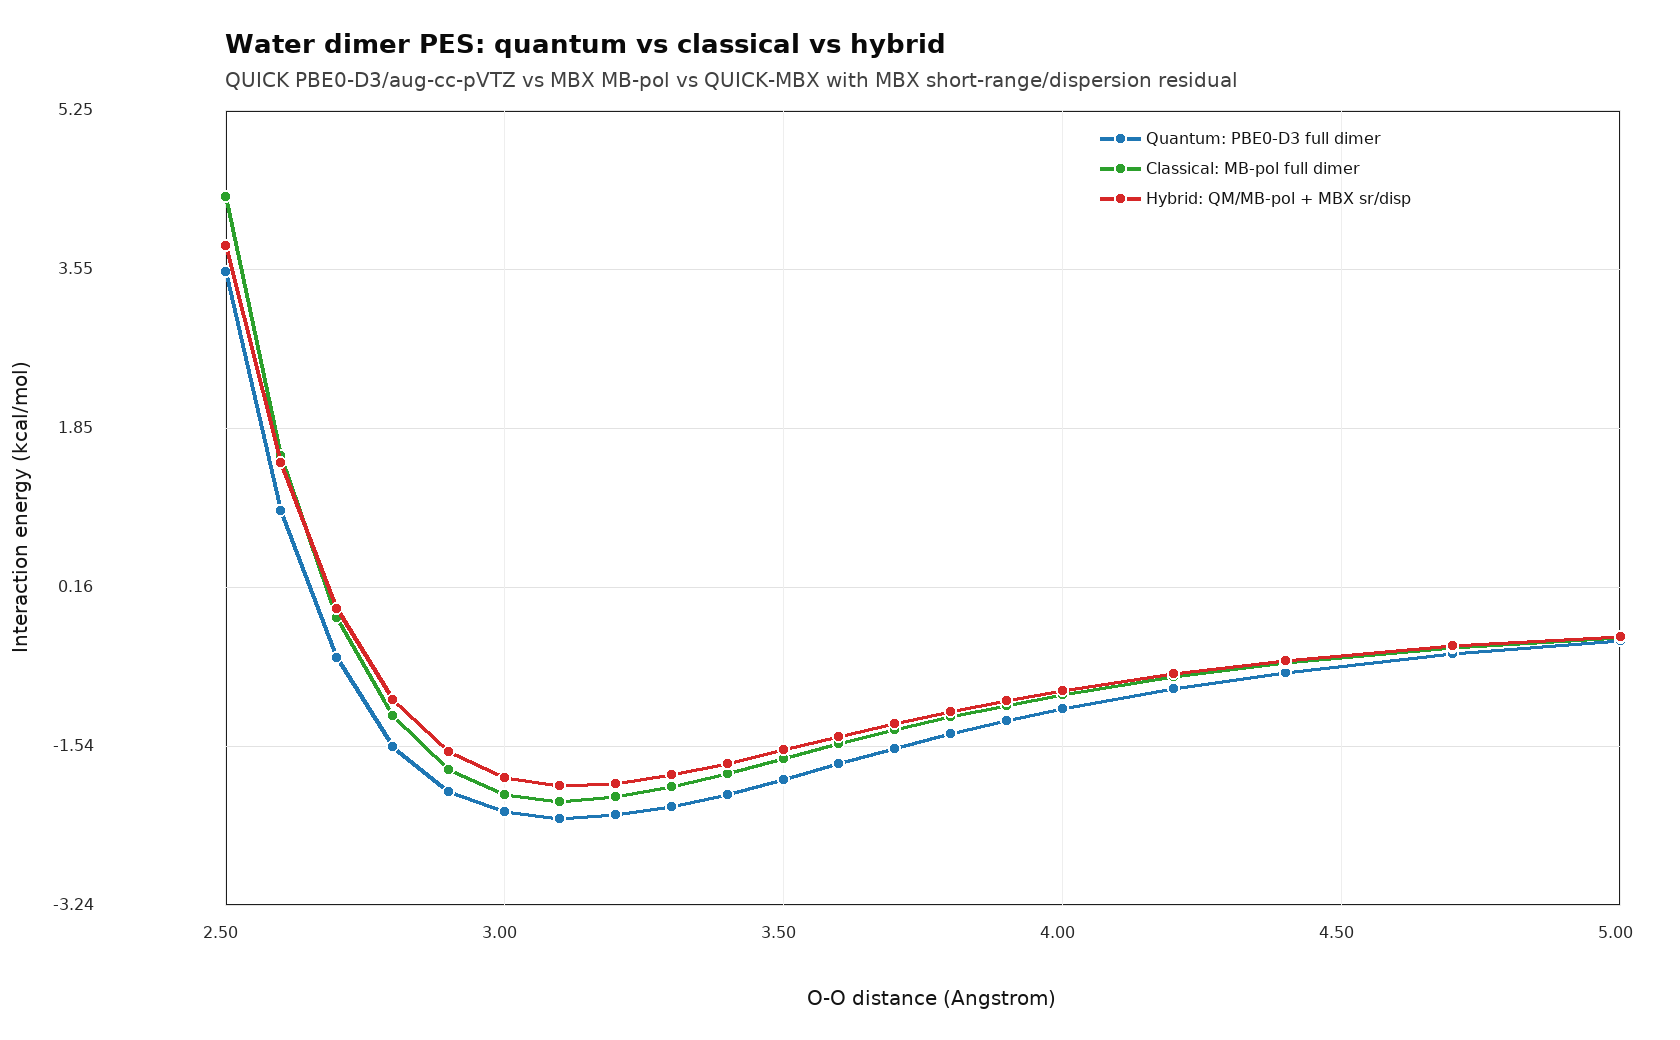
\includegraphics[width=0.96\linewidth]{lambros_dimer_three_way_augccpvtz_20pt_srdisp_corrected.png}
  \caption{Water-dimer interaction-energy scan on identical XYZ points.
  The hybrid curve is the complete current QM/MB-pol validation energy:
  QUICK PBE0-D3 for monomer $A$, MBX MB-pol electrostatics and
  polarization for monomer $B$, plus the MBX h2o/h2o short-range and
  dispersion residual.}
  \label{fig:water_dimer_scan}
\end{figure}

Representative points from the 20-point PBE0-D3/aug-cc-pVTZ scan are:

\begin{tabular}{rrrrrr}
\toprule
$R_{\rm OO}$ (\AA) & PBE0-D3 & MB-pol & raw hybrid &
$\Delta E_{\rm sr/disp}$ & corrected hybrid \\
\midrule
2.50 &  3.525636 &  4.318132 & -11.442793 & 15.243055 &  3.800262 \\
3.10 & -2.309084 & -2.128275 &  -3.089691 &  1.123305 & -1.966385 \\
5.00 & -0.418826 & -0.385009 &  -0.352831 & -0.017670 & -0.370501 \\
\bottomrule
\end{tabular}

All energies in this table are interaction energies in kcal/mol. The
raw column is retained only as a diagnostic decomposition, not as a
complete QM/MM method. The
corrected hybrid now has the expected qualitative behavior: a repulsive
short-range wall, an attractive near-minimum point, and a long-range tail
that decays with the full QM and full MB-pol curves. The corrected hybrid
does not yet prove quantitative production accuracy, but it removes the
unphysical flipped curve observed with electrostatic/polarization coupling
alone.

\subsection{MB-pol-optimized MB-PBE water-dimer scan}

MBX also provides an \texttt{mbpbe} water model, effectively an MB-pol-like
potential trained against a PBE-D3 reference. This makes it a useful
classical partner for a PBE-D3/MB-PBE QUICK--MBX validation. The local MBX
installation contains an \texttt{optimize} executable, but that executable
is unconstrained and would relax all scan points toward ordinary dimer
minima. For a potential-energy scan, the O--O separation must remain fixed.

A lightweight constrained MBX-gradient optimizer was therefore added:
\begin{itemize}
  \item \texttt{optimize\_water\_dimer\_mbx\_scan.py} calls MBX analytic
    gradients through the local MBX Python binding, projects the gradient
    onto the tangent space of the fixed O(1)--O(4) distance, and relaxes
    the remaining Cartesian degrees of freedom with a small projected
    L-BFGS optimizer.
  \item \texttt{run\_mbpbe\_water\_scan.py} consumes that XYZ stack and
    evaluates five fixed-geometry interaction curves: full QUICK
    PBE-D3/aug-cc-pVTZ, full MB-pol, full MB-PBE, corrected
    PBE-D3/MB-pol, and corrected PBE-D3/MB-PBE.
\end{itemize}

The MB-PBE hybrid required one adapter-level ABI fix. MBX's legacy
\texttt{initialize\_system\_} entry point uses fixed five-character C
buffers for monomer names, which is enough for \texttt{h2o} but not for
\texttt{mbpbe} plus a null terminator. QUICK now calls MBX's existing
\texttt{initialize\_system\_py\_} entry point, which accepts \texttt{char**}
name arrays and therefore passes \texttt{mbpbe} without modifying MBX.

The dimer residual convention is the same as
Eq.~\ref{eq:mbpol_sr_disp_residual}. For MB-pol the residual baseline sets
\texttt{ignore\_2b\_poly = [[h2o,h2o]]} and
\texttt{ignore\_dispersion = [[h2o,h2o]]}. For MB-PBE the corresponding
baseline sets \texttt{ignore\_2b\_poly = [[mbpbe,mbpbe]]} and
\texttt{ignore\_dispersion = [[mbpbe,mbpbe]]}. The corrected hybrid curves
therefore include the MBX short-range and dispersion cross residual rather
than showing only the raw electrostatic/polarization coupling.

\begin{figure}[htbp]
  \centering
  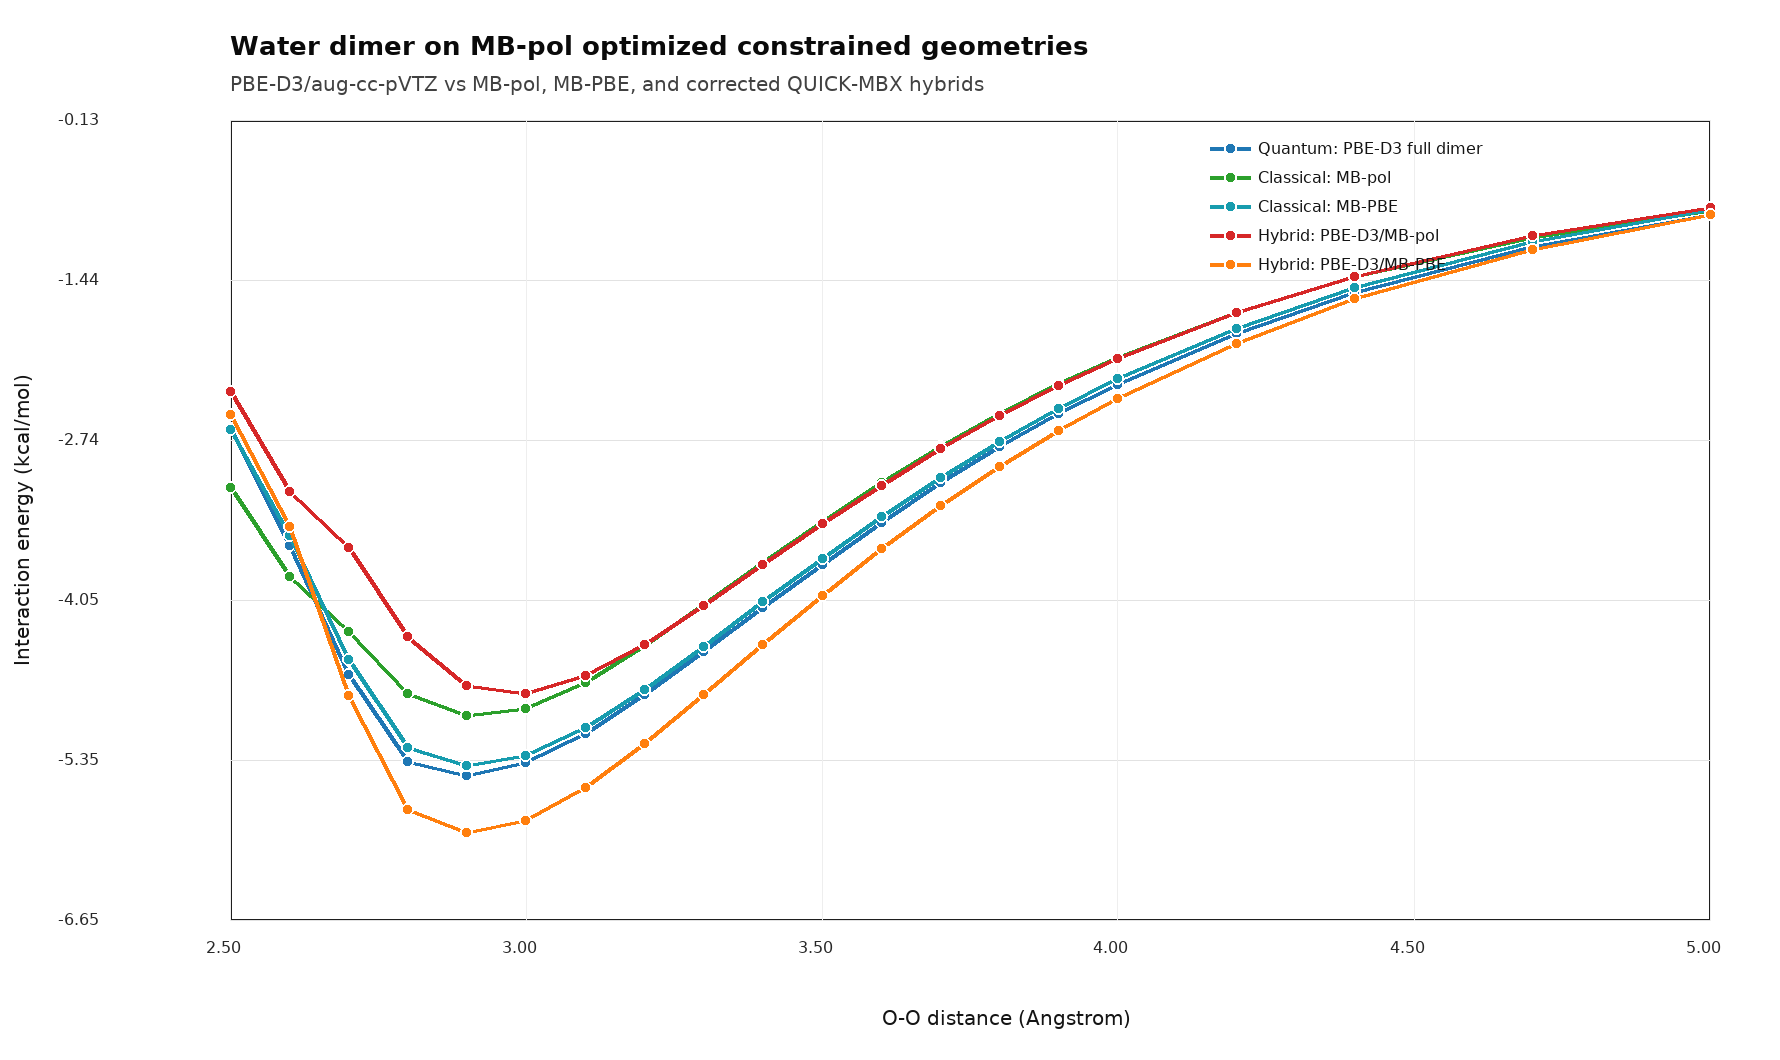
\includegraphics[width=0.96\linewidth]{water_dimer_mbpolopt_pbe_d3_mbpbe_20pt.png}
  \caption{Twenty-point water-dimer interaction-energy scan on MB-pol
  optimized constrained geometries. Each point fixes $R_{\rm OO}$ and
  relaxes the remaining coordinates with MB-pol before evaluating QUICK
  PBE-D3/aug-cc-pVTZ, full MB-pol, full MB-PBE, corrected
  PBE-D3/MB-pol, and corrected PBE-D3/MB-PBE energies.}
  \label{fig:mbpbe_water_mbpolopt_scan}
\end{figure}

\begin{tabular}{rrrrrr}
\toprule
$R_{\rm OO}$ & PBE-D3 & MB-pol & MB-PBE & PBE-D3/MB-pol & PBE-D3/MB-PBE \\
\midrule
2.50 & -2.650359 & -3.132446 & -2.657764 & -2.349579 & -2.536994 \\
2.90 & -5.477824 & -4.988697 & -5.392890 & -4.739664 & -5.940941 \\
5.00 & -0.903218 & -0.869014 & -0.863688 & -0.847918 & -0.904959 \\
\bottomrule
\end{tabular}

All energies in the table are interaction energies in kcal/mol. The 20
MB-pol constrained geometries were generated in about 13 seconds and all
points satisfied the projected-force acceptance criterion
(\texttt{max force < 5e-4} kcal mol$^{-1}$ \AA$^{-1}$ or
\texttt{RMS force < 2.5e-4} kcal mol$^{-1}$ \AA$^{-1}$). On these relaxed
geometries, MB-PBE tracks the full PBE-D3 curve more closely than MB-pol.
The target PBE-D3/MB-PBE hybrid is slightly overbound near the minimum but
has a smooth well and a long-range tail that nearly coincides with PBE-D3.
The PBE-D3/MB-pol curve is retained as a reference hybrid with the original
MB-pol water model.

The production commands were:
\begin{verbatim}
export QUICK_BUILD=/private/tmp/quick-build-mbx-focktest
export CODEX_PY=/Users/etiennepalos/.cache/codex-runtimes/\
codex-primary-runtime/dependencies/python/bin/python3

cmake --build $QUICK_BUILD \
  --target quick test-api-mbx-water-xyz-scan --parallel 8

python3 validation/quick_mbx/optimize_water_dimer_mbx_scan.py \
  --max-steps 600 --force-tol 5.0e-4

$CODEX_PY validation/quick_mbx/run_mbpbe_water_scan.py \
  --scan-exe $QUICK_BUILD/src/test-api-mbx-water-xyz-scan \
  --xyz validation/quick_mbx/water_dimer_mbpol_optimized_20pt.xyz \
  --csv validation/quick_mbx/water_dimer_mbpolopt_pbe_d3_mbpbe_20pt.csv \
  --output validation/quick_mbx/water_dimer_mbpolopt_pbe_d3_mbpbe_20pt.png
\end{verbatim}

\subsection{Troubleshooting the MB-PBE hybrid overbinding}

The first MB-PBE hybrid scan is scientifically useful because full
PBE-D3 and full MB-PBE agree closely, while the corrected
PBE-D3/MB-PBE hybrid is still modestly overbound near the minimum.  This
rules out a simple ``MB-PBE is the wrong classical reference'' explanation.
The current corrected hybrid interaction curve is
\begin{equation}
  E_{\rm hyb}^{\rm current}
  =
  E_{\rm raw}^{\rm QM/MBPBE}
  +
  \Delta E_{\rm sr/disp}^{\rm MBPBE},
  \qquad
  \Delta E_{\rm sr/disp}^{\rm MBPBE}
  =
  E_{\rm full}^{\rm MBPBE}
  -
  E_{\rm base}^{\rm MBPBE}.
\end{equation}
Here $E_{\rm raw}^{\rm QM/MBPBE}$ is the self-consistent QUICK/MBX
electrostatic-polarization baseline, while $E_{\rm base}^{\rm MBPBE}$ is
the MB-PBE electrostatic-polarization baseline obtained by disabling the
water--water 2B polynomial and dispersion.  The MB-PBE short-range and
dispersion residual was trained to correct $E_{\rm base}^{\rm MBPBE}$, not
the modified baseline $E_{\rm raw}^{\rm QM/MBPBE}$.  The diagnostic
baseline-mismatch term is therefore
\begin{equation}
  \delta_{\rm base}
  =
  E_{\rm raw}^{\rm QM/MBPBE}
  -
  E_{\rm base}^{\rm MBPBE}.
\end{equation}

Subtracting this term gives a baseline-aligned diagnostic curve,
\begin{equation}
  E_{\rm hyb}^{\rm aligned}
  =
  E_{\rm hyb}^{\rm current}
  -
  \delta_{\rm base}.
\end{equation}
For this two-water validation case the aligned diagnostic is numerically
equivalent to replacing the cross electrostatic-polarization baseline by
the MB-PBE baseline before adding the MB-PBE residual.  It is therefore
not yet a production QM/MM energy model; it is a bookkeeping diagnostic
that isolates why the current hybrid overbinds.

\begin{figure}[htbp]
  \centering
  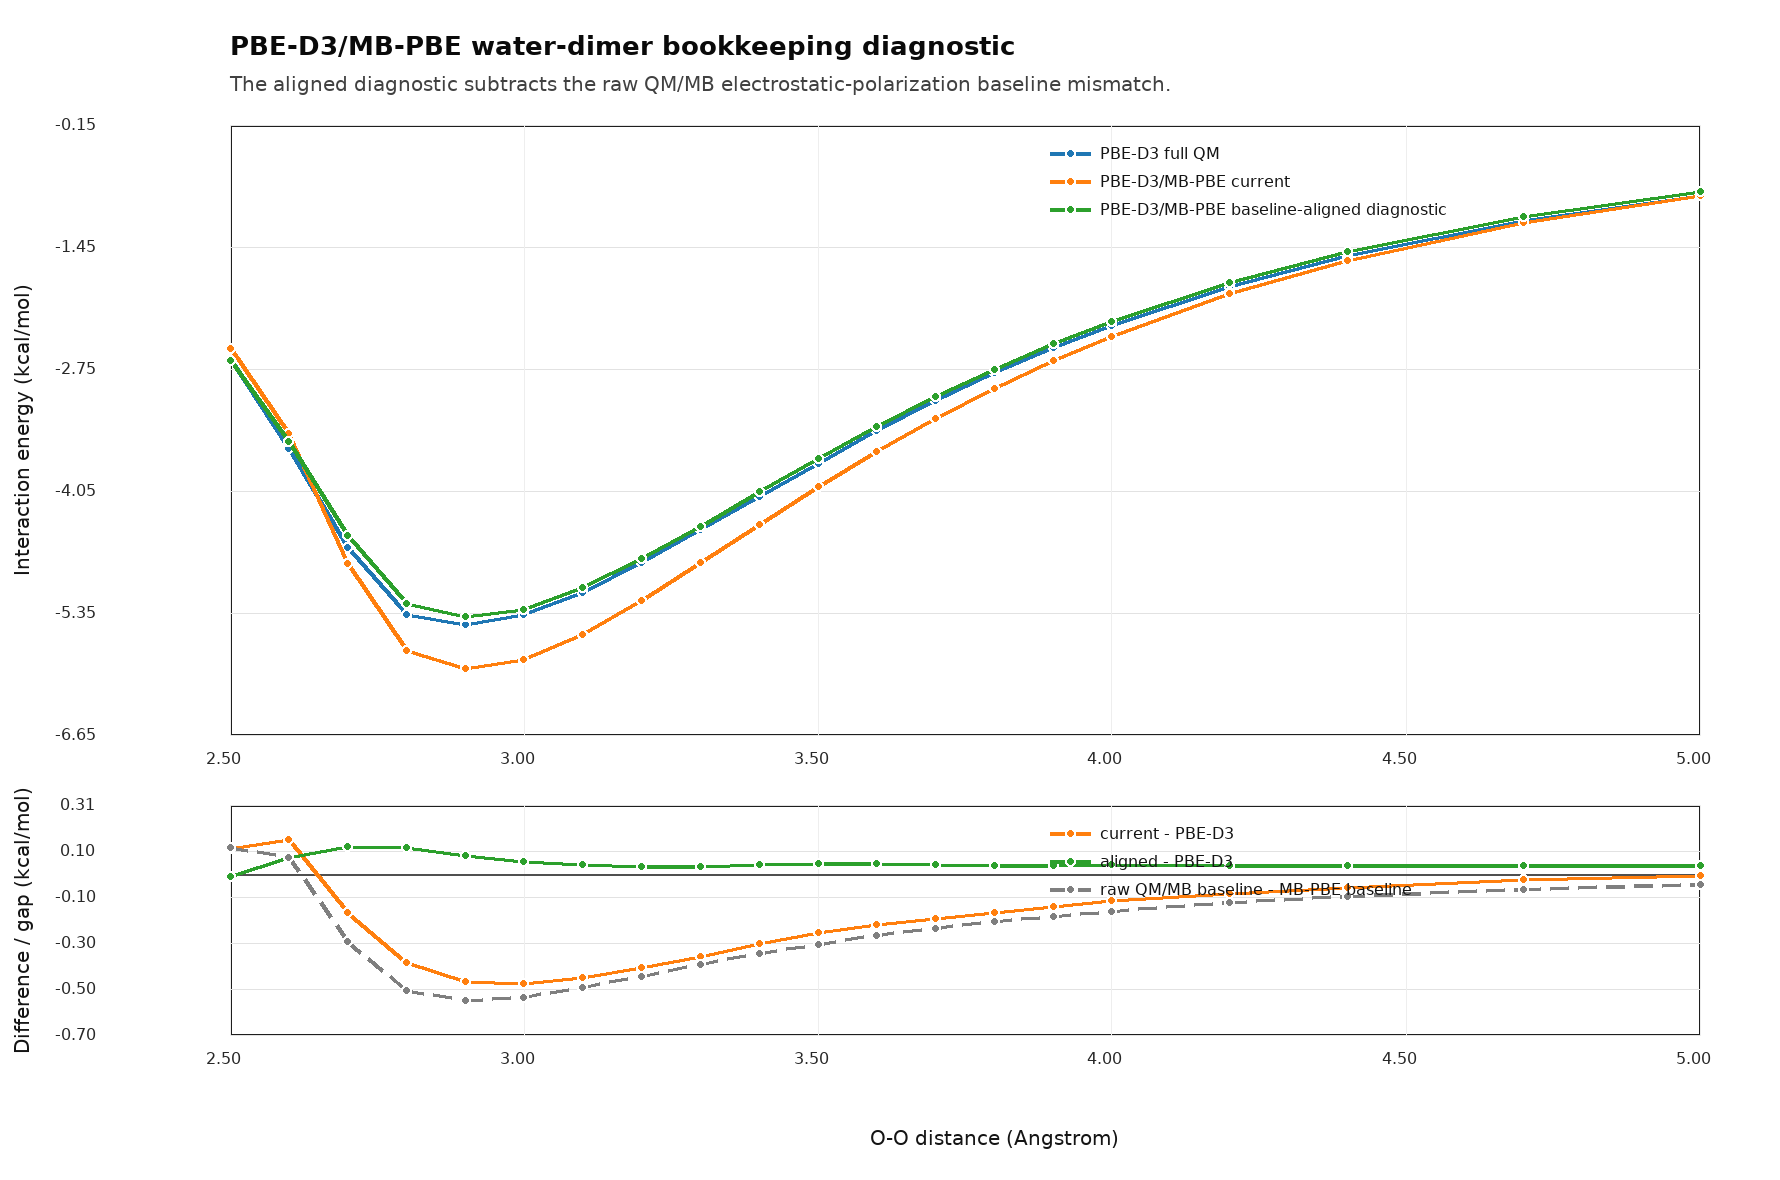
\includegraphics[width=0.96\linewidth]{water_dimer_mbpbe_bookkeeping_diagnostic.png}
  \caption{Bookkeeping diagnostic for the MB-PBE water-dimer scan.  The
  current PBE-D3/MB-PBE hybrid overbinding tracks the raw
  QM/MB electrostatic-polarization baseline mismatch relative to the
  MB-PBE baseline.  Removing that mismatch reduces the 20-point RMS error
  against PBE-D3 from 0.269 to 0.060 kcal/mol.}
  \label{fig:mbpbe_bookkeeping_diagnostic}
\end{figure}

Three-point Hamiltonian-scale diagnostics support the same conclusion.
Removing the induced-dipole Fock operator changed the 2.90~\AA{} error
only from $-0.46$ to $-0.42$ kcal/mol, so induced coupling is not the
dominant source.  Removing the permanent-site Fock operator moved the
2.90~\AA{} error to $+0.28$ kcal/mol, and a half-scale permanent operator
gave $-0.27$ kcal/mol while worsening the short-range point.  Thus a
constant scale is not an acceptable production fix.  The production path
should instead implement a physically motivated permanent-electrostatics
damping or charge-penetration correction, or obtain an MBX component API
for a QM/MM-specific short-range residual that is trained or evaluated
against the actual QM/MB electrostatic-polarization baseline.

\subsection{Small pair scans beyond water}

The same residual workflow was extended to three additional small-pair
checks. Methane--methane uses the MBX
\texttt{040\_ch4-ch4\_mb-nrg\_2bnb} example with five MBX sites per
methane. The residual baseline disables
\texttt{ignore\_2b\_poly = [[ch4,ch4]]} and
\texttt{ignore\_dispersion = [[ch4,ch4]]}. The H2O--CH4 scan uses the MBX
\texttt{042\_ch4-h2o\_mb-nrg\_2bnb} example with
\texttt{ignore\_2b\_poly = [[ch4,h2o]]} and
\texttt{ignore\_dispersion = [[ch4,h2o]]}. The Cl-/H2O scan uses the MBX
\texttt{022\_h2o-cl\_mb-nrg\_2bnb} example with
\texttt{ignore\_2b\_poly = [[cl-,h2o]]} and
\texttt{ignore\_dispersion = [[cl-,h2o]]}.

\begin{figure}[htbp]
  \centering
  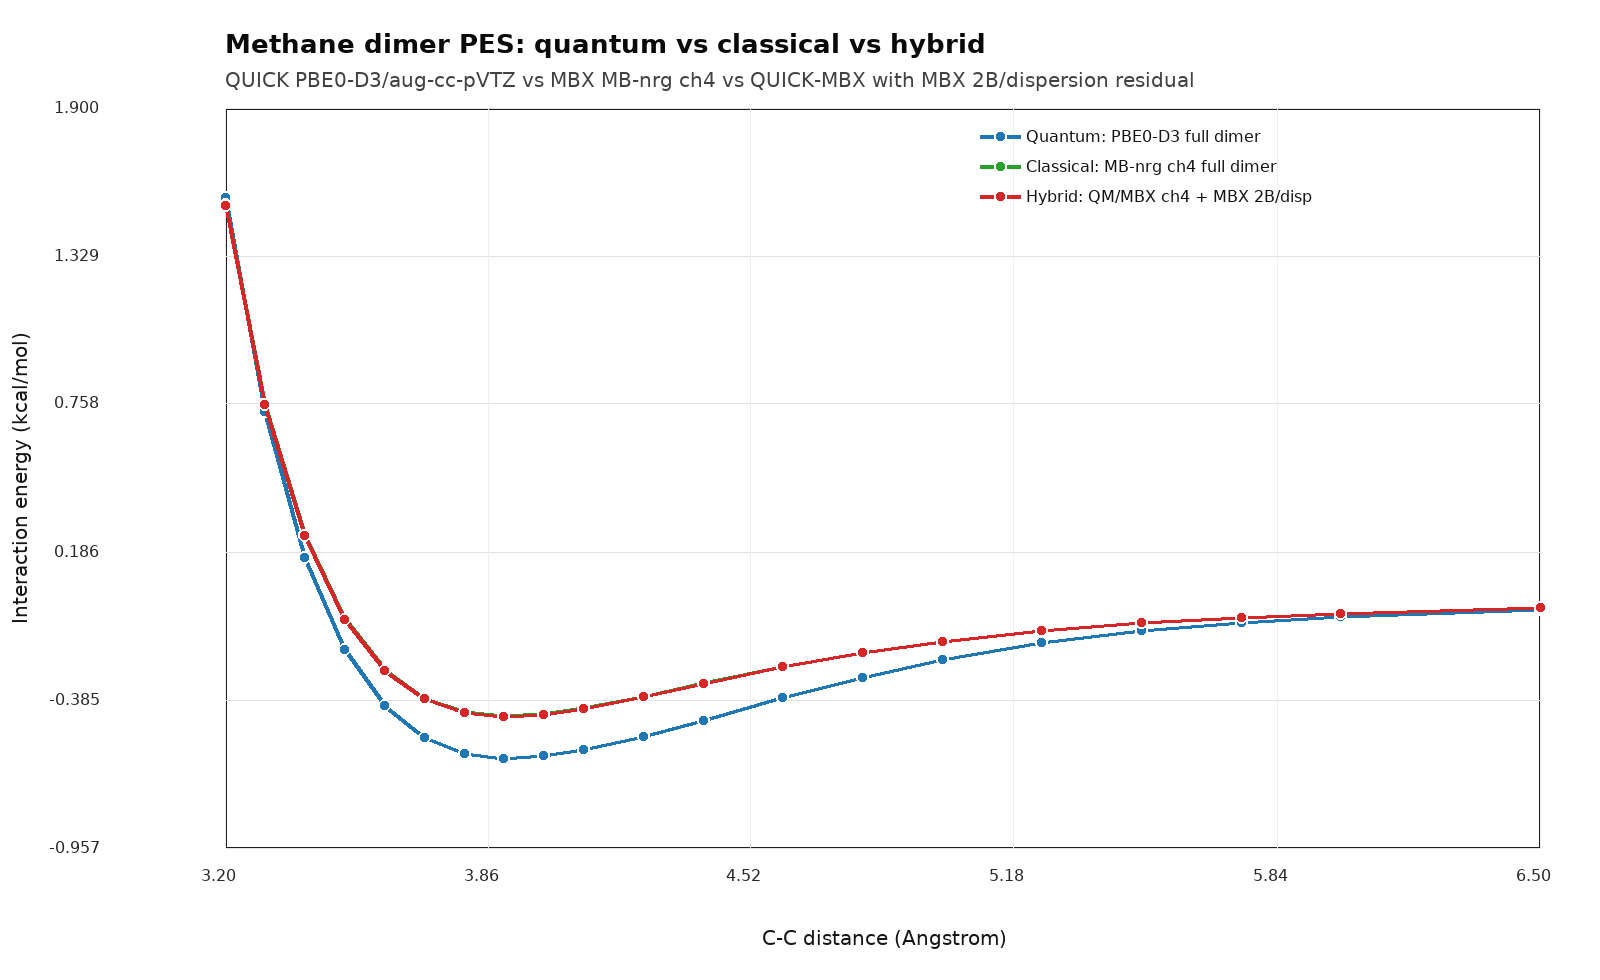
\includegraphics[width=0.92\linewidth]{ch4_dimer_three_way_augccpvtz_20pt_srdisp_corrected.png}
  \caption{Twenty-point methane-dimer scan. The corrected hybrid curve is
  QUICK PBE0-D3/aug-cc-pVTZ on monomer A, MBX MB-nrg methane on monomer B,
  plus the isolated ch4/ch4 two-body and dispersion residual.}
  \label{fig:ch4_dimer_scan}
\end{figure}

\begin{figure}[htbp]
  \centering
  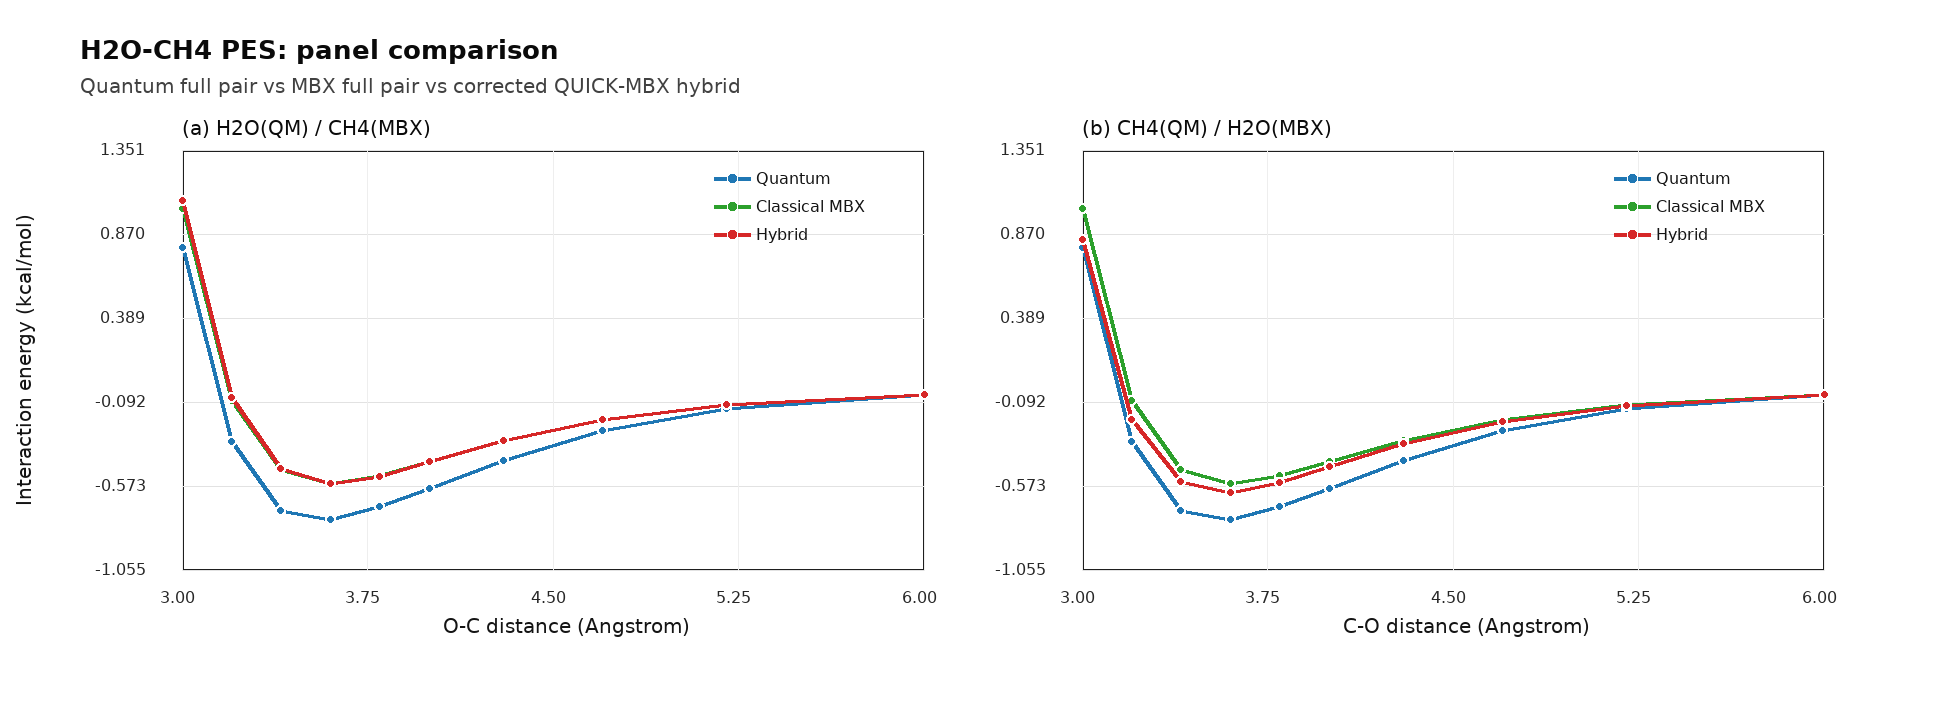
\includegraphics[width=\linewidth]{h2o_ch4_two_panel_augccpvtz_10pt_srdisp_corrected.png}
  \caption{Ten-point H2O--CH4 role-swap scan. Panel (a) treats H2O as QM
  and CH4 as MBX; panel (b) treats CH4 as QM and H2O as MBX. Both panels
  use the same MBX ch4/h2o two-body and dispersion residual.}
  \label{fig:h2o_ch4_scan}
\end{figure}

\begin{figure}[htbp]
  \centering
  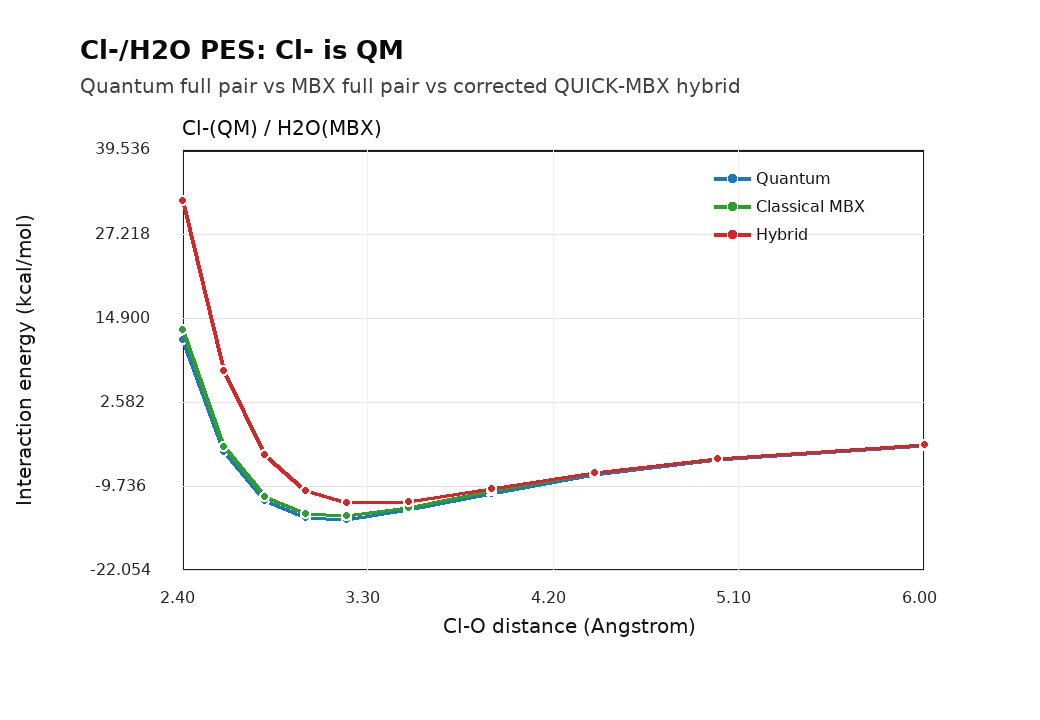
\includegraphics[width=0.76\linewidth]{cl_h2o_cl_qm_augccpvtz_10pt_srdisp_corrected.png}
  \caption{Ten-point Cl-/H2O scan with Cl- as the QM subsystem. The
  corrected hybrid uses the MBX cl-/h2o short-range and dispersion
  residual. The short-range wall is over-repulsive at the first point, so
  this ionic case is a useful stress test rather than a quantitative
  acceptance result.}
  \label{fig:cl_h2o_scan}
\end{figure}

\begin{figure}[htbp]
  \centering
  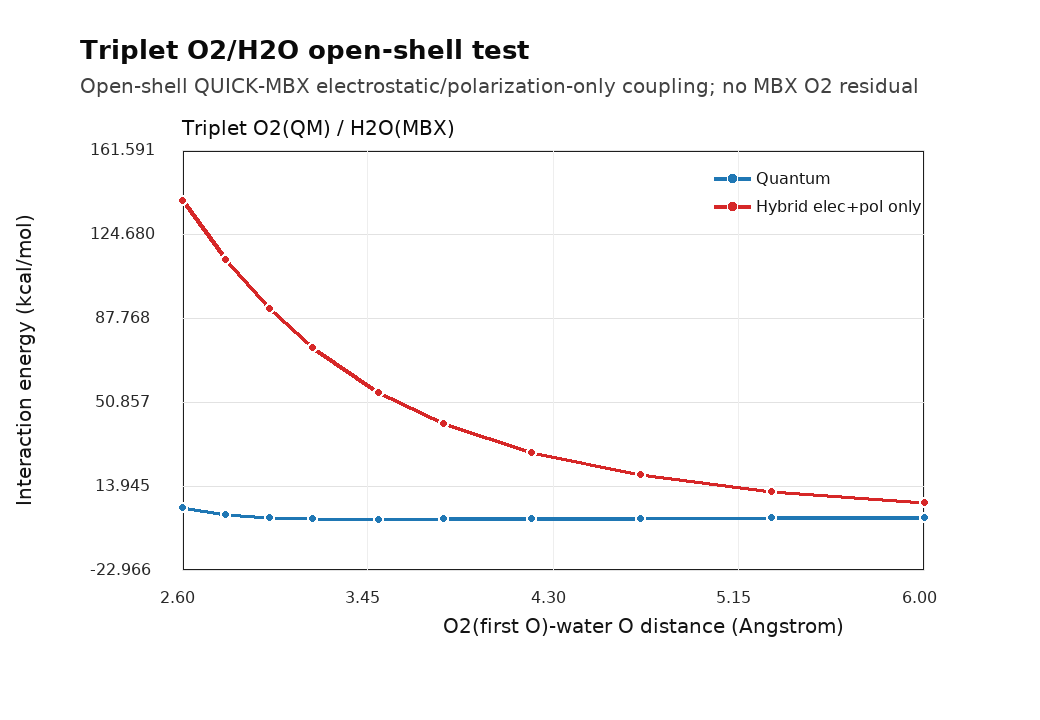
\includegraphics[width=0.76\linewidth]{o2_h2o_triplet_augccpvtz_10pt_open_shell.png}
  \caption{Ten-point triplet O2/H2O open-shell smoke test. QUICK runs the
  O2-containing calculations as unrestricted triplets. No MBX O2 model or
  O2/H2O residual is available in the local MBX tree, so the red curve is
  electrostatic/polarization coupling only and is not a complete QM/MM
  method.}
  \label{fig:o2_h2o_scan}
\end{figure}

\begin{table}[htbp]
  \centering
  \small
  \begin{tabular}{llrlrrrr}
    \toprule
    System & QM fragment & Points & Residual & $R_{\rm min}$ &
    PBE0-D3 & MBX & Hybrid \\
    \midrule
    CH4--CH4 & CH4 & 20 & 2B/disp & 3.90 & -0.610 & -0.447 & -0.448 \\
    H2O--CH4 & H2O & 10 & 2B/disp & 3.60 & -0.763 & -0.560 & -0.559 \\
    H2O--CH4 & CH4 & 10 & 2B/disp & 3.60 & -0.763 & -0.560 & -0.608 \\
    Cl-/H2O & Cl- & 10 & 2B/disp & 3.20 & -14.588 & -14.095 & -12.183 \\
    O2/H2O & triplet O2 & 10 & none & 6.00 & -0.033 & N/A & 6.769 \\
    \bottomrule
  \end{tabular}
  \caption{Representative minima from the additional scans. Distances are
  in Angstrom and energies are interaction energies in kcal/mol. The
  ``Hybrid'' column is the corrected hybrid where an MBX cross residual can
  be isolated; for O2/H2O it is the electrostatic/polarization-only
  diagnostic.}
  \label{tab:small_pair_scan_summary}
\end{table}

The CH4--CH4 and H2O--CH4 scans give the desired qualitative publication
behavior: a short-range wall, an attractive minimum, and a tail that
decays toward zero. The corrected hybrid follows the corresponding MBX
curve closely for methane and closely tracks the mixed H2O--CH4 MBX
reference after the residual is added. The Cl-/H2O scan also converges and
has the expected well and tail, but the first short-range point is too
repulsive relative to both PBE0-D3 and the MBX ion-water model. This should
be revisited before using ionic systems as an acceptance benchmark. The
triplet O2/H2O case verifies the unrestricted open-shell path and MBX water
coupling, but because no O2 cross residual is available it is not a
complete chemical validation.

\subsection{Trimer roadmap}

A trimer scan was not attempted in this resource window. For a future
water-trimer validation with monomer $A$ in QUICK and monomers $B,C$ in
MBX, the cross residual should be isolated explicitly rather than silently
mixing MB-only and QM/MB terms. A practical MBX-derived residual is
\begin{equation}
  \Delta E_{\rm cross}^{ABC}
  =
  \left[
    E_{\rm full}^{ABC}-E_{\rm elec+pol}^{ABC}
  \right]
  -
  \left[
    E_{\rm full}^{BC}-E_{\rm elec+pol}^{BC}
  \right].
\end{equation}
The first bracket contains all non-electrostatic residual terms in the
trimer, while the second removes the purely MBX $B$--$C$ residual already
belonging to the MBX internal environment. A 2B-only correction should
disable only h2o/h2o two-body polynomial and dispersion terms. Any 3B
short-range correction must be isolated and reported separately by also
controlling the h2o/h2o/h2o three-body polynomial term.

When QUICK is configured with \texttt{-DMBX=TRUE}, CMake also builds optional
\texttt{test-api-mbx} and \texttt{test-api-mbx.MPI} smoke executables. These
initialize one and two MB-pol waters through
\texttt{setQuickMBXWaterSystem}, run fixed-geometry energy-only QUICK SCF
calculations with \texttt{MBX\_QMMM}, check SCF convergence, and print
parseable total energies. The validation driver runs them automatically when
the executables are present or when paths are supplied with
\texttt{--quick-mbx-smoke} and \texttt{--quick-mbx-smoke-mpi}. The next
validation cases should be:
\begin{itemize}
  \item QUICK-generated ESP/EFIELD at MBX sites compared to a controlled
    point-charge reference.
  \item More fixed-geometry QM/MB-pol water monomer/dimer geometries, kept
    small enough for routine laptop validation.
\end{itemize}

\section{Roadmap toward gradients and MD}

EFG is not required for the first energy-only QM/MB-pol target, but it is
needed for analytic gradients and MD. Stage 4 provides a CPU finite-
difference total-gradient reference and a tiny MD smoke test. Stage 4.5
adds a decomposition diagnostic showing that MBX internal forces plus the
QUICK permanent site-gradient term recover most of the MBX-side total
finite-difference gradient for the tiny water test. Production analytic
QM/MB-pol gradients still require:
\begin{itemize}
  \item Derivatives of QUICK ESP and EFIELD at MBX sites with respect to QM
    nuclear coordinates, including direct analytic AO field-operator
    derivatives rather than finite differences of point-charge operators.
  \item A MBX external-derivative ABI that accepts the QUICK field-gradient
    tensor and any induced-dipole response data needed by MBX's external
    induced-gradient machinery.
  \item Component-consistent gradients for the same energy bookkeeping used
    in Eq.~\ref{eq:quick_mbx_additive} and for any MBX short-range/
    dispersion residual added to a corrected hybrid validation energy.
  \item Consistent redistribution of MBX site gradients to real atoms,
    validated for virtual sites and lone-pair sites.
  \item Explicit tests that the QUICK field-gradient convention
    $G_{ij}=\partial E_i/\partial C_j$ is used throughout.
\end{itemize}

The next QUICK-side development step is to promote the permanent
$-q_s\mathbf{E}^{\rm QM}(\mathbf{C}_s)$ MBX-site gradient and MBX
redistribution path from diagnostic code into an analytic gradient
component, with finite-difference regression tests on fixed water
geometries. The highest-value QUICK-side refactor after that is a direct
analytic AO field-operator derivative contraction that shares recurrence
tables with EFIELD/EFG. The highest-value MBX-side interface improvement
is an external-call wrapper that exposes and validates external
field-gradient handoff without requiring QUICK to vendor or patch MBX
locally.

\section*{References}

\begin{itemize}
  \item Lambros, E.; Lipparini, F.; Cisneros, G. A.; Paesani, F. A
    many-body, fully polarizable approach to QM/MM simulations. J. Chem.
    Theory Comput. 2020, 16, 7462--7472.
    DOI: 10.1021/acs.jctc.0c00932.
  \item The OpenMMPol Library for Polarizable QM/MM Calculations of
    Properties and Dynamics. 2024. \url{https://arxiv.org/abs/2401.14691}.
  \item MBX source and documentation. \url{https://github.com/paesanilab/MBX}.
\end{itemize}

\end{document}
